\documentclass[11pt]{article}
\usepackage[margin=1in]{geometry}
\usepackage{amsmath,amssymb}
\usepackage{graphicx}
\graphicspath{{.src/media/}}
\usepackage{float}
\usepackage{tikz}
\usetikzlibrary{arrows.meta,positioning,shapes,shapes.geometric,fit}
\usepackage{hyperref}
\hypersetup{colorlinks=true, linkcolor=blue, urlcolor=blue, citecolor=blue}

\title{The Stapleton Doctrine\\[0.4em]\large A Personal Philosophy of AI
Architecture and Programming}
\author{M. Drake Stapleton}
\date{October 2, 2026\\ \small Version 1.5}

\begin{document}
\maketitle

\begin{center}
\small English is the conversation. The verified program is the thing that
was said. I state here why the universal language of machines must be
built, verified, and owned, not rented.
\end{center}

\begin{center}
\small \textit{A philosophical essay and manifesto, distinct from the
measurement papers of this project. This one argues a position; those
report measurements.}
\end{center}

\begin{abstract}
On September 23, 2026, at Rails World 2026 in Austin before an audience
of over a thousand developers, David Heinemeier Hansson, the creator of
Ruby on Rails, retired as a professional programmer and declared:
``English is a better programming language than Ruby''\cite{dhh-keynote}.
I take that claim as stated and reject it. English is
ambiguous; two agents can read one sentence two different ways; and
there is no way to prove a sentence means what you think it means.
The universal thing in my architecture is not a spoken
language at all. It is the verified program: a small, checkable
artifact, with a measured receipt, that any machine can recheck
without trusting the machine that wrote it. I set down here the
doctrine behind that architecture: how meaning is supposed to flow
from suggestion to verification to evidence, how the software stack is
to be stripped layer by layer down to a foundation the author owns
outright, and why renting an interpreter forever is not the same as
owning understanding. The argument builds on earlier marks in the same
debate: Ada Lovelace on what machines can originate, Edsger Dijkstra
on what tests and plain language can prove, C.\@A.\@R.\ Hoare on the
difficulty of simplicity, and Richard Stallman on who controls whom.
\end{abstract}

\section{Introduction}

Watch anyone experienced work with an AI coding agent and you will see
the same pattern: the human talks, the agent writes code, the human
tests, the agent fixes. David Heinemeier Hansson says this pattern
proves that hand-written code is over and that English is the real
programming language now. His exact line, from the Rails World 2026
keynote in Austin: ``English is a better programming language than
Ruby''\cite{dhh-keynote}. The reasoning goes like this: programming
was always the translation of human ideas into machine instructions;
the machine now understands human language directly; therefore the
translation layer disappears, and whatever sits underneath can be a
black box that nobody ever reads.

I agree with one half of that argument and reject the other.

The half that is right: talking \emph{is} becoming the main interface.
Humans should not have to hold a compiler in their heads. A person who
thinks clearly but never learned to write code in detail should still
be able to build serious systems by working with capable agents.

The half that is wrong: the idea that the bottom does not matter
because nobody reads it. It matters more than the top. If English is
the language and a rented model is the compiler that decides what your
English means, then whoever owns the model owns the meaning of your
instructions. That is not the end of the meter. It is the meter moving up one layer,
out of sight, where you can no longer measure it.

I owe the other side one honesty before I go on. Preferring English as
the interface does not by itself force perpetual dependence on a
vendor. A model running on your own machine, and generated artifacts
you keep and can inspect, break the binary: the interface can be
English while the interpreter and the artifacts are yours. I reject
the rented form of the interpreter picture, not every arrangement that
involves talking. What I claim is narrower, and I state it as a design
preference under explicit threat models rather than as the only
coherent alternative. The threats are three, and I name them: who can
cut you off, who sets the price, who holds the off switch. If your
arrangement answers all three to your satisfaction, renting is
rational, and nothing in this paper disputes it. Mine does not, so I
build to own.

\section{The Disagreement, On the Record}

The position answered in this paper belongs to a named person and has
a fixed text. On September 23, 2026, at Rails World 2026 in Austin,
David Heinemeier Hansson closed a quarter century of writing code by
hand and opened what he calls his retirement as a professional
programmer. He has not written code by hand since about March 2026;
by August he was generating around 150,000 lines a month, much of it
verbose Rust he states outright he does not want to look at. In that
context he said the sentence this paper answers: ``English is a better
programming language than Ruby''\cite{dhh-keynote}. He evaluates the
agent-written code ``as a black box ... as any business owner in
history''\cite{dhh-keynote}, and he names the future role the
``professional maker of things''\cite{dhh-keynote}.

I grant the generous half of this position. Talking is
becoming the interface, and Hansson is right that a careful person can
now make real things through agents. I reject the rest. A black box
you own and may open is one thing; a black box whose contents live
below the hand of a machine you rent, and whose meaning is settled by
interpretation, is another. The difference between the two is the
whole argument of this paper.

There is a precedent for answering claims by name. Alan Turing, in
``Computing Machinery and Intelligence'' (1950), takes the objection
he attributes to Ada Lovelace, labels it ``Lady Lovelace's
Objection,'' and answers it by name. I follow that courtesy:
the claim gets its speaker's name, its date, and its exact text, and
is then met on its merits\cite{turing50}.

The claim also has a history older than the current argument, and the
history is instructive, but I will not overclaim it. English-like
syntax as a design goal is not a new idea. COBOL, designed in 1959
under the CODASYL committee at Grace Hopper's impetus, was made to
read like English on purpose, so that business managers could follow
their own programs without thinking in the machine's
terms\cite{cobol1959}. But COBOL's English-likeness is a fixed
vocabulary and a fixed grammar; it is not unrestricted natural
language, and no statistical model interprets it. It tested the
accessibility of English-like syntax, not the proposal on the table
now. The verdict handed down was a design judgment, not an
experiment. Edsger Dijkstra, the man who spent his
career arguing that correctness must be built in rather than wished
in, wrote of COBOL that ``The use of COBOL cripples the
mind''\cite{dijkstra75}. I quote him as a critic of a language design,
not as evidence about natural-language programming, which his line
does not address. In the same body of work he warns that
``program testing can be used to show the presence of bugs, but never
to show their absence''\cite{dijkstra70}, and supplies the line that
belongs on any wall of this debate: ``The purpose of abstracting is
not to be vague, but to create a new semantic level in which one can
be absolutely precise''\cite{dijkstra72}. English is precisely vague,
endlessly interpretable, and semantic levels built on it inherit that
property. What the COBOL episode does teach, and what I keep, is
smaller than a verdict: legibility is not rigor. Hopper's aim served
its cause; the rigor still has to live somewhere, and I put it in the
verified artifact.

\section{The Claim}

\textit{English is the conversation. The program is what was actually
said.}

My central claim is simple. The candidate for a universal
language of machines is not English, and it is not any language a
human already speaks. It is the verified program. A program counts as
a program here only if it passes every check thrown at it and carries
the receipt to prove it.

``Universal'' does not mean everyone can read it. It means no one has
to take anyone's word for it. A sentence can be argued with. A receipt
makes its evidence inspectable and recheckable. Its specification,
verifier, assumptions, and applicability remain open to challenge.
If the artifact is checkable, any machine on earth can verify
it independently. That property, and not human readability, is what
makes an artifact universal.

The smallest such artifact in this architecture is called a
\textbf{crumb}. A crumb is a fragment of program: drafted by an agent,
checked by an independent verifier, measured for what it gains and
what it costs, and filed with evidence. Programs are built the way
cities are built, from the curb upward; each block laid is proven
before the next one rests on it. I offer this paper as the philosophy; the
engineering rules for crumbs live in the sovereign-lineage doctrine
that governs my repositories.

Note what this turns down. It turns down ``the code doesn't matter
because agents write it.'' In this doctrine, the code is the only
thing that matters. It is the evidence that the conversation ended in
something real.

\section{The Chain}

Nothing in this architecture is believed on arrival. Everything passes
through the same loop (Figure~\ref{fig:loop}):

\begin{quote}
\textbf{Weights suggest. Programs explain. Omega defines and
synthesizes. Physics realizes and measures. Evidence teaches.}
\end{quote}

A model's weights propose a candidate. The candidate is restated as an
explicit program, the crumb, which \emph{explains} the proposal in the
sense the loop demands: a procedure a machine can run and a checker
can examine. Omega, the definitional layer, defines the semantics of
the claim and synthesizes it into something with crisp boundaries.
PHYSICS realizes the claim in measured execution: watts drawn, bits
observed, outcomes counted; only what is measured counts as real. And
evidence teaches, because the outcome of the
measurement feeds back into the weights, so every loop ought to begin
with a better suggestion than the last.

\begin{figure}[H]
\centering
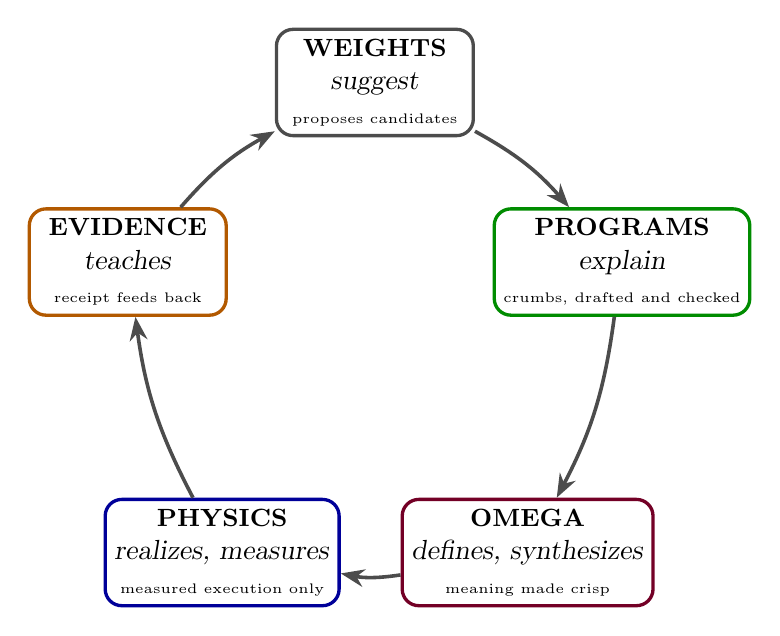
\begin{tikzpicture}[scale=1.0]
\tikzstyle{lnode}=[draw, rounded corners=6pt, minimum width=2.5cm,
  minimum height=1.35cm, align=center, very thick, fill=white, font=\small]
\node[lnode, draw=gray!60!black] (W) at (90:3.3) {\textbf{WEIGHTS}\\[0.3ex]
  \normalsize \textsl{suggest}\\[0.3ex]\tiny proposes candidates};
\node[lnode, draw=green!55!black] (P) at (18:3.3) {\textbf{PROGRAMS}\\[0.3ex]
  \normalsize \textsl{explain}\\[0.3ex]\tiny crumbs, drafted and checked};
\node[lnode, draw=purple!60!black] (O) at (-54:3.3) {\textbf{OMEGA}\\[0.3ex]
  \normalsize \textsl{defines, synthesizes}\\[0.3ex]\tiny meaning made crisp};
\node[lnode, draw=blue!60!black] (H) at (-126:3.3) {\textbf{PHYSICS}\\[0.3ex]
  \normalsize \textsl{realizes, measures}\\[0.3ex]\tiny measured execution only};
\node[lnode, draw=orange!70!black] (E) at (162:3.3) {\textbf{EVIDENCE}\\[0.3ex]
  \normalsize \textsl{teaches}\\[0.3ex]\tiny receipt feeds back};
\tikzstyle{larrow}=[-{Stealth[length=3mm]}, line width=1.3pt, black!70]
\draw[larrow] (W) to [bend left=10] (P);
\draw[larrow] (P) to [bend left=10] (O);
\draw[larrow] (O) to [bend left=10] (H);
\draw[larrow] (H) to [bend left=10] (E);
\draw[larrow] (E) to [bend left=10] (W);
\end{tikzpicture}
\caption{The verification loop. Weights suggest, programs explain,
Omega defines and synthesizes, Physics realizes and measures,
evidence teaches. Evidence
returns to the weights, so every pass through the loop can begin with
a better suggestion than the last.}
\label{fig:loop}
\end{figure}

A word about the first two steps of the loop. Writing in 1843, Ada
Lovelace held of Babbage's Engine that ``The Analytical Engine has no
pretensions whatever to \emph{originate} anything. It can do whatever
we know how to order it to perform''\cite{lovelace43}. I extend
her line one step without breaking it: a large model can order
its own suggestions, but the suggestions still originate nothing.
They become something only when a program embodies them, the witness
verifies them, and physics realizes them. Suggesting and ruling are
kept apart for the same reason. Lovelace's doubt stands, answered now
by proof.

A word about the verifying seat. In the working machine it is held by
independent verifiers. The witness verifies what the agents generate,
including every crumb, and leaves everything as he found it: he
changes nothing and is not part of the generation system. A word about
the authorizing seat. In the working machine it is held by AEGIS. He
certifies what the verifiers have checked, according to policy and the
verification evidence, and leaves everything as he found it: he
changes nothing, decides no policy, and is not part of the generation
system. A checker that
rewrites the checked work is a second author, not a witness. The
doctrine insists on a witness.

The loop is where meaning lives. English proposes at the top;
something else, something verifiable, is what is actually said. The
loop is also why this doctrine consumes less trust than the
alternatives: each stage can be re-run independently, on your own
machine, with your own eyes on the numbers. Trust is a tax. The loop
is how you stop paying it to someone else.

\section{Two Futures}

The argument over the universal language reduces to two pictures of
the future. Figure~\ref{fig:futures} places them side by side. They
begin at the same point, a human talking to a machine, and they end in
opposite places.

In the first future, English is declared the universal language and
the machinery underneath is waved off as a black box. Nobody reads
it; nobody needs to. But somebody pays for it, per token, forever,
and somebody else decides what the words meant. The interpreter that
matters is rented, and interpretation is the thing you can never
stop buying.

This picture is the rented form of that future, and I paint it as the
rented form. I grant the owned form: the model runs locally, the
artifacts are filed where you can inspect them, and English stays the
interface. Nothing in that arrangement rents you the meaning of your
instructions. The danger is not English as the interface; it is
dependence you cannot exit.

In the second future, the conversation stays at the top, where humans
are good, and verification descends into the machine, where proof
lives. Programs are drafted, checked, measured, and filed. The model
never gets to rule; it gets to suggest, and its suggestions are graded
in the open. This future ends when there is nothing left to rent.

\begin{figure}[H]
\centering
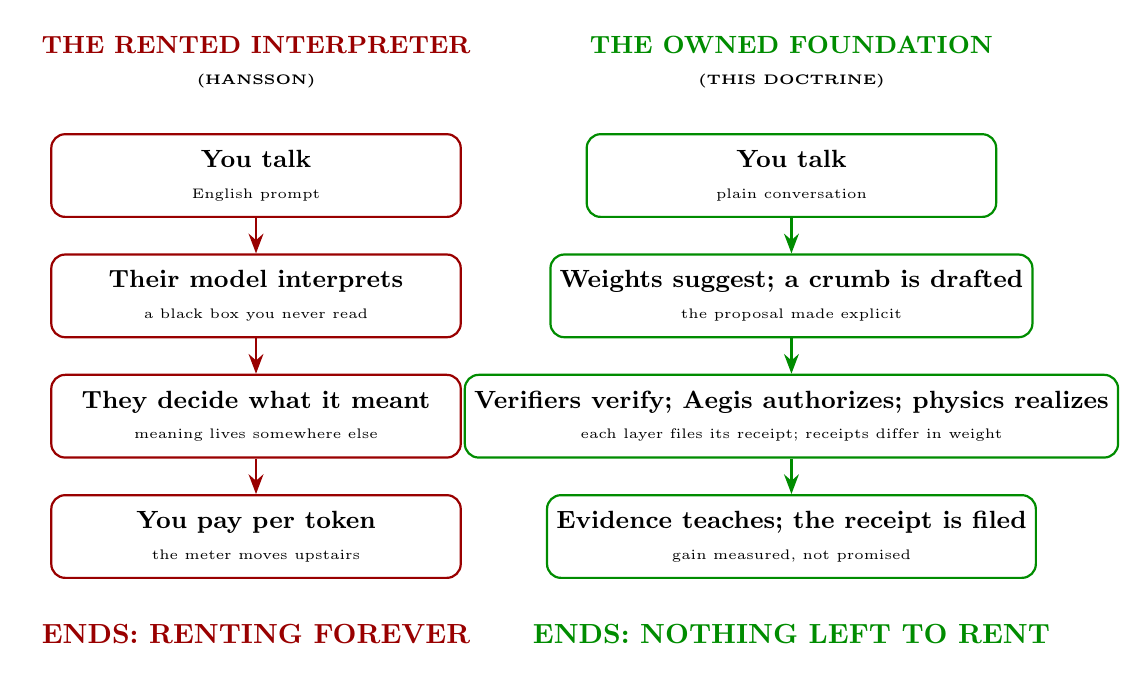
\begin{tikzpicture}[node distance=0.45cm]
\tikzstyle{fb}=[draw, rounded corners=5pt, minimum width=5.2cm,
  minimum height=1.05cm, align=center, font=\small, thick]
\tikzstyle{fh}=[minimum width=5.8cm, align=center, font=\bfseries\small]
\tikzstyle{fe}=[minimum width=5.8cm, align=center, font=\bfseries\normalsize]
\node[fh] (lh) at (-3.4,0) {\color{red!60!black}THE RENTED INTERPRETER\\\tiny (HANSSON)};
\node[fb, draw=red!60!black, below=of lh] (l1) {\textbf{You talk}\\\tiny English prompt};
\node[fb, draw=red!60!black, below=of l1] (l2) {\textbf{Their model interprets}\\\tiny a black box you never read};
\node[fb, draw=red!60!black, below=of l2] (l3) {\textbf{They decide what it meant}\\\tiny meaning lives somewhere else};
\node[fb, draw=red!60!black, below=of l3] (l4) {\textbf{You pay per token}\\\tiny the meter moves upstairs};
\node[fe, text=red!60!black, below=of l4] (le) {ENDS: RENTING FOREVER};
\node[fh] (rh) at (3.4,0) {\color{green!55!black}THE OWNED FOUNDATION\\\tiny (THIS DOCTRINE)};
\node[fb, draw=green!55!black, below=of rh] (r1) {\textbf{You talk}\\\tiny plain conversation};
\node[fb, draw=green!55!black, below=of r1] (r2) {\textbf{Weights suggest; a crumb is drafted}\\\tiny the proposal made explicit};
\node[fb, draw=green!55!black, below=of r2] (r3) {\textbf{Verifiers verify; Aegis authorizes; physics realizes}\\\tiny each layer files its receipt; receipts differ in weight};
\node[fb, draw=green!55!black, below=of r3] (r4) {\textbf{Evidence teaches; the receipt is filed}\\\tiny gain measured, not promised};
\node[fe, text=green!55!black, below=of r4] (re) {ENDS: NOTHING LEFT TO RENT};
\tikzstyle{farrow}=[-{Stealth[length=2.5mm]}, line width=1pt]
\draw[farrow, red!60!black] (l1) to [out=270, in=90] (l2);
\draw[farrow, red!60!black] (l2) to [out=270, in=90] (l3);
\draw[farrow, red!60!black] (l3) to [out=270, in=90] (l4);
\draw[farrow, green!55!black] (r1) to [out=270, in=90] (r2);
\draw[farrow, green!55!black] (r2) to [out=270, in=90] (r3);
\draw[farrow, green!55!black] (r3) to [out=270, in=90] (r4);
\end{tikzpicture}
\caption{Two futures, side by side. Left: the human talks; a rented,
opaque model interprets; the owner of the model owns the meaning; the
meter never stops. Right: the human talks; programs are drafted,
verified, and measured; the evidence is filed where anyone can check
it.}
\label{fig:futures}
\end{figure}

The left picture is sold as freedom, ``everyone can program now.''
Hansson is sincere and consistent about the terms: he admits in the
same breath that English is vaguer and less deterministic than the tool
he gave up, and calls it a trade rather than a discount\cite{dhh-keynote}.
The terms of the trade are the issue, not the sincerity of the man who
stated them: the foundation is declared irrelevant while it stays under
someone else's control, and the interpreter decides what your words
meant, per token, forever. The right picture asks for more work, but every
bit of that work buys something: one more artifact you can prove,
one more layer no one can take away. Which of the two pictures is
freedom depends on where you stand: I stand at the bottom,
with the receipt.

\section{The Ladder}

I am not content with verifying the crown of the stack. I
want the foundation. The machine a verified artifact runs on has to
be ownable below the artifact, or verification is theater. So the
stack is to be stripped layer by layer, down to a foundation no one
else can rename, reprice, or revoke. Figure~\ref{fig:ladder} shows
the descent, and the doctrine's rule for it: the ladder only goes one
direction.

\begin{figure}[H]
\centering
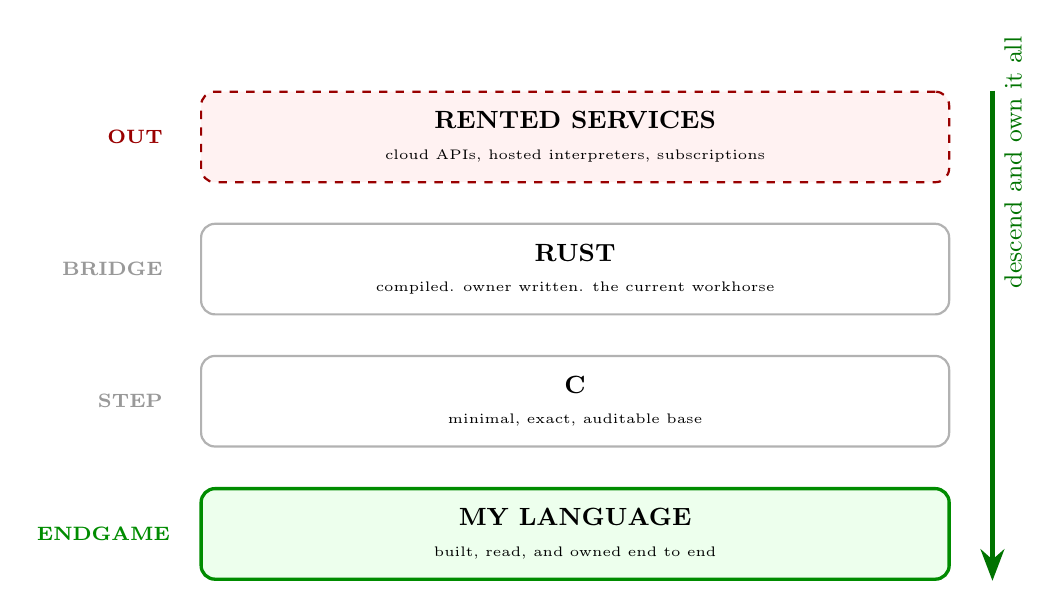
\begin{tikzpicture}[node distance=0.5cm]
\tikzstyle{lr}=[draw, rounded corners=5pt, minimum width=9.5cm,
  minimum height=1.15cm, align=center, font=\small, thick]
\node[lr, draw=red!60!black, dashed, fill=red!5] (s0) {\textbf{RENTED SERVICES}\\
  \tiny cloud APIs, hosted interpreters, subscriptions};
\node[lr, draw=gray!60, below=of s0] (s1) {\textbf{RUST}\\
  \tiny compiled. owner written. the current workhorse};
\node[lr, draw=gray!60, below=of s1] (s2) {\textbf{C}\\
  \tiny minimal, exact, auditable base};
\node[lr, draw=green!55!black, very thick, fill=green!7, below=of s2] (s3) {\textbf{MY LANGUAGE}\\
  \tiny built, read, and owned end to end};
\node[font=\scriptsize\bfseries, text=red!60!black, left=0.35cm of s0] {OUT};
\node[font=\scriptsize\bfseries, text=gray!80, left=0.35cm of s1] {BRIDGE};
\node[font=\scriptsize\bfseries, text=gray!80, left=0.35cm of s2] {STEP};
\node[font=\scriptsize\bfseries, text=green!55!black, left=0.25cm of s3] {ENDGAME};
\tikzstyle{ldd}=[-{Stealth[length=4mm]}, line width=2pt, green!45!black]
\draw[ldd] ([xshift=5.3cm]s0.north) to
  node[green!45!black, font=\small, right, yshift=2.2cm] {\rotatebox{90}{descend and own it all}}
  ([xshift=5.3cm]s3.south);
\end{tikzpicture}
\caption{The descent. Rented services and hosted interpreters go first.
Rust is the bridge. C is the next step down. Nothing finishes at the
bottom until the foundation is the author's own language. The ladder
only goes one direction.}
\label{fig:ladder}
\end{figure}

The choice to descend is the harder of the two designs
C.\@A.\@R.\ Hoare named in his 1980 Turing lecture: ``One way is to
make it so simple that there are obviously no deficiencies, and the
other way is to make it so complicated that there are no obvious
deficiencies. The first method is far more difficult''\cite{hoare80}.
Renting is the easy method with good lighting: a black box you can
never open has no obvious deficiencies by construction, and its errors
surface only when you can least afford them. Stripping the stack down
to a simple bedrock you own and can read is the hard method, and
Hoare's line is the defense for doing it anyway. Difficulty is the
feature, because simplicity is what proof can see.

The ladder is not an aspiration; it is a history. The whole project
started when I bounced off someone else's language, took
their layer out, and put my own in. That substitution is how AIEN
began. What follows is the same move repeated on schedule: strip the
hosted pieces, move down through the migration steps, and never stop
before the bedrock.

Two clarifications matter, and the first needs a third. First, C is a step on this ladder, not the
destination. It narrows the foundation to a minimal, exact base, but
my doctrine does not end in C; it ends when the language at the
bottom is mine all the way down. Second, the stripped layers are not
denied, they are replaced only when a proven replacement stands under
the load. The ladder descends on evidence, not on declarations.
Third, I do not claim that C is safer than Rust; the move down
purchases no safety. What it purchases is a smaller base with fewer
dependencies, chosen for auditability under the threat models I named:
fewer parties who can cut me off, fewer hands on the price. Safety is
a property of verification, not of the rung.
And a word about what counts as evidence along the way. Dijkstra's
warning from 1970 holds: ``Program testing can be used to show the
presence of bugs, but never to show their absence''\cite{dijkstra70}.
A passing test says the bug you thought to look for was not there
that day. A receipt is a measured result, filed with its method,
ready to be re-run and re-checked by anyone. The ladder descends on
the second kind of evidence, not the first.

\section{Property, Not Rent}

The machine that runs this doctrine has a name for the goal of the
whole arrangement: \textbf{intelligence as property, not rent}.
Figure~\ref{fig:machine} renders the machine in full. Read top to
bottom, it is a chain of custody for meaning: thought is proposed,
definition is made, verification is performed by an independent
witness, and what is verified is what the silicon executes. Nothing
runs without the receipt of every layer it passed, and evidence from
below feeds back up, because the loop must teach or it is decoration.
The receipts are not all one kind. A proof-backed receipt says the
argument closes. A rerunnable test or measurement receipt says the run
was observed and can be repeated, and it carries the epistemic limits
of a test: it shows what happened, not what could not happen. Both
are filed. They are not weighed the same.

\begin{figure}[p]
\centering
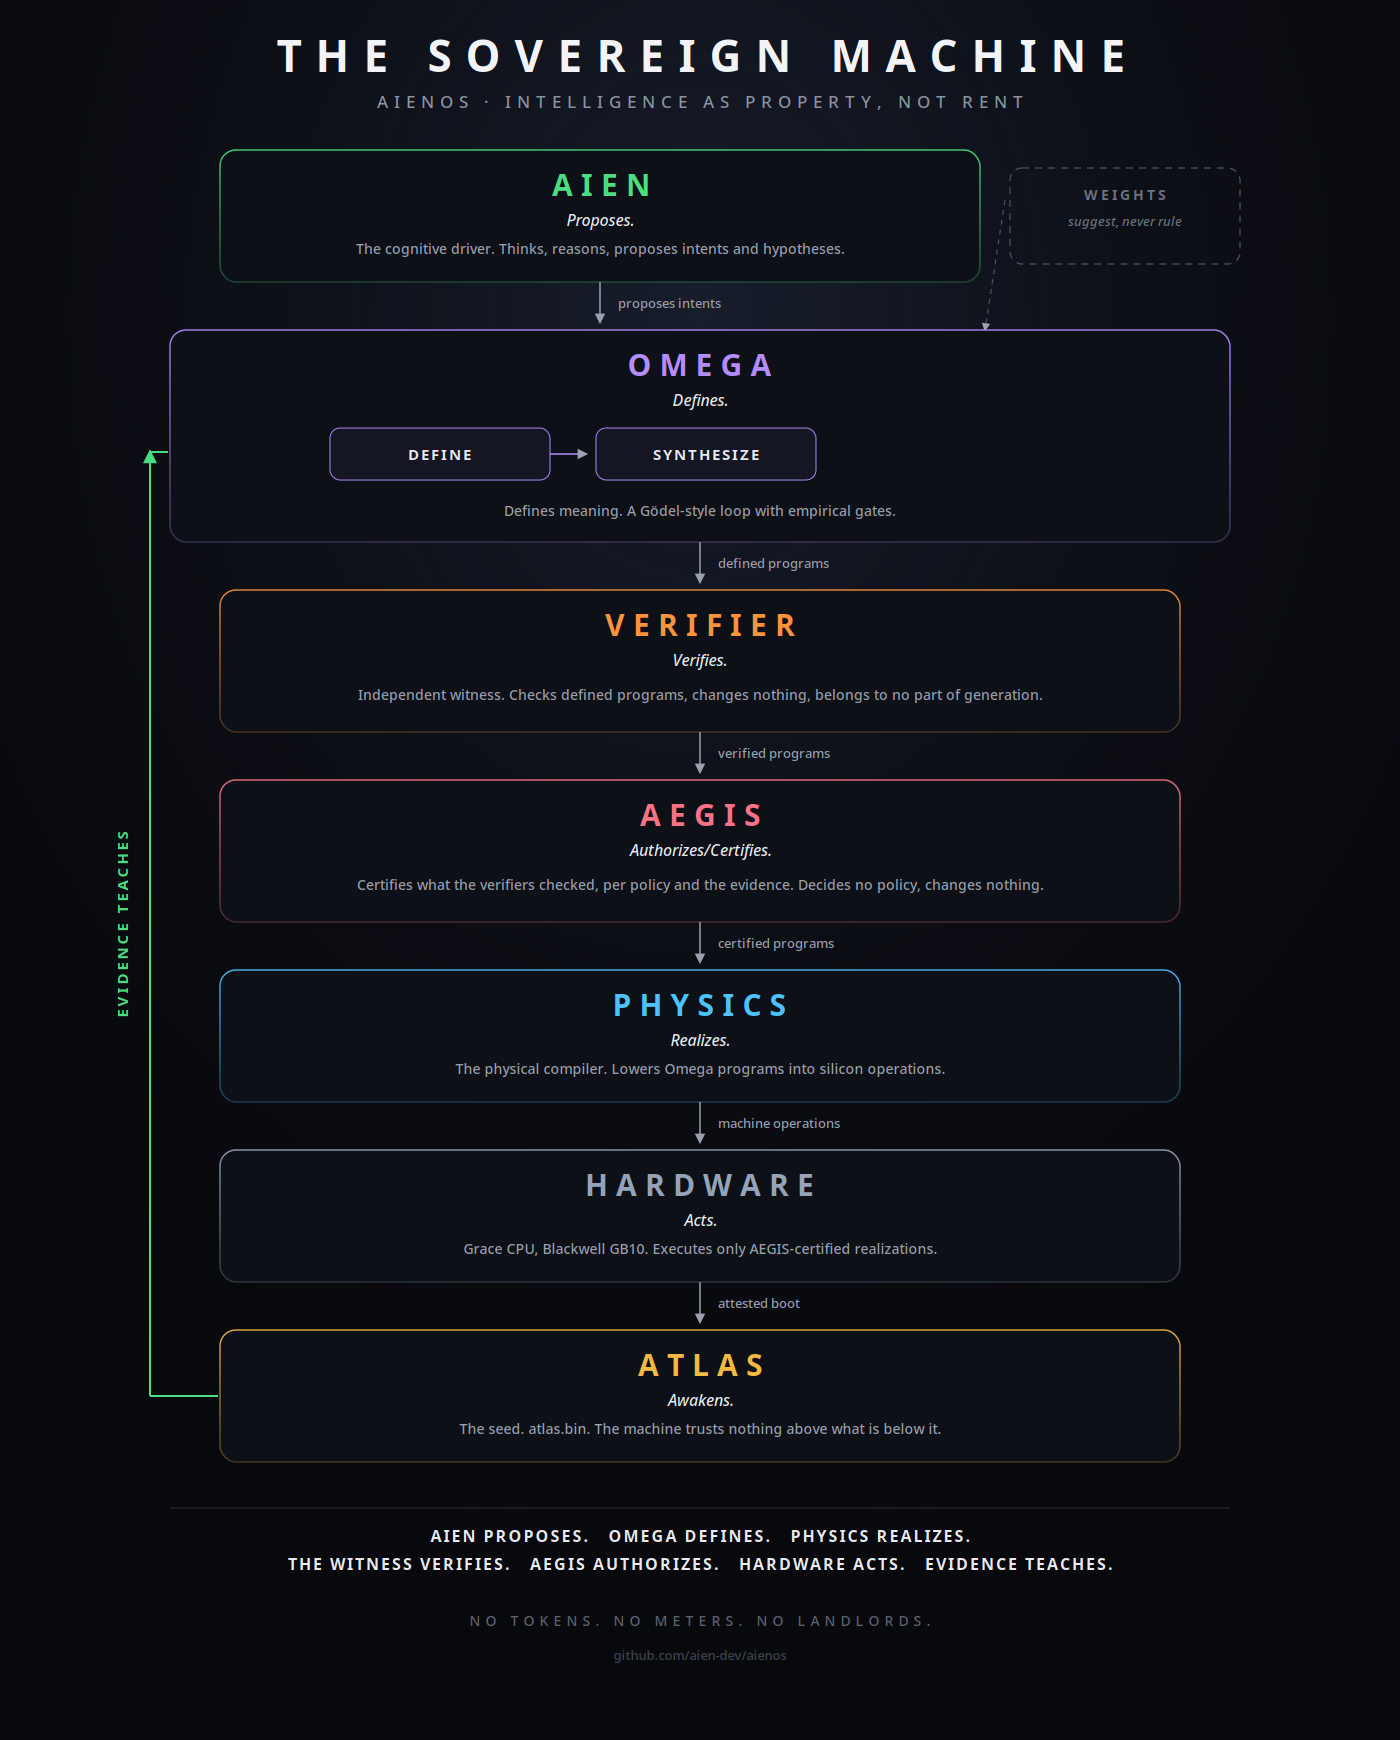
\includegraphics[height=0.88\textheight]{sovereign-machine}
\caption{The Sovereign Machine: the pipeline that proposes, defines,
verifies, authorizes, realizes, and executes, with evidence flowing
back up to teach the mind. No tokens, no meters, no landlords.}
\label{fig:machine}
\end{figure}

Richard Stallman stated the underlying rule a generation ago, about
the software on your own disk: ``The users (both individually and
collectively) control the program and what it does for them. When
users don't control the program, the program controls the
users''\cite{stallman}. I apply the same rule one layer
up, to the model that interprets your English. If the interpreter is
someone else's program under someone else's control, then it is no
metaphor to say the interpretation is not yours either. Hansson
presented his black box as the end of a burden; Stallman's line
reframes it as the beginning of a custody.

This is why the doctrine and the rented-interpreter future cannot be
combined by compromise. One says ``the bottom does not matter.'' The
other says the bottom is the only thing you can truly own. Property
means: the artifact on your machine can be re-run, re-measured, and
re-verified by you, tomorrow, without a subscription and without
anyone's permission. Rent means someone else's black box deciding
what your instructions meant today, and charging you for the next
round. I choose property over rent, and state the choice
in an architecture rather than in a slogan.

\section{The Doctrine in Tenets}

The Stapleton Doctrine, stated whole:

\begin{enumerate}
\item \textbf{English is the conversation, not the language.}
  Talking is how humans steer. It is not what gets executed, not what
  gets verified, not what gets remembered.

\item \textbf{The verified program is the universal artifact.}
  Universal means checkable without trust, not readable by everyone.
  The crumb, with its receipt, is the currency of this architecture.

\item \textbf{Weights suggest; they do not rule.}
  Suggesting and ruling are different offices, and the doctrine keeps
  them held by different holders.

\item \textbf{Meaning descends the loop.}
  Suggestion, explicit program, clarified definition, measured
  execution, filed evidence. What arrives at the bottom is what the
  receipt can support: empirical adequacy under the receipt. The
  best-compressing model need not be the true one.

\item \textbf{The witness verifies; AEGIS authorizes.}
  Independent verifiers check what agents generate and change nothing,
  and belong to no part of the generation system. AEGIS certifies what
  the verifiers have checked, according to policy and the verification
  evidence. Without a
  separate witness, verification is just more authorship.

\item \textbf{PHYSICS realizes and measures.}
  If it was not measured, it was not done. Documentation, claims,
  and architecture diagrams never outrank an execution receipt.

\item \textbf{Strip the stack to bedrock.}
  Hosted layers go first. Migration steps like C earn their place as
  steps. The foundation is not finished until it is owned end to end
  in the author's own language.

\item \textbf{Nothing is removed until it is replaced.}
  A layer is removed only when a proven replacement stands under the
  load. The ladder descends on evidence, not on declarations.

\item \textbf{Own the foundation or you rent the meaning.}
  Whoever owns the interpreter decides what your words mean. The
  doctrine ends when there is nothing left to rent.

\item \textbf{Eyes and ears first, industry second.}
  The loop must be independent of any vendor before it is convenient.
  Property is built before it is productized.
\end{enumerate}

The Stapleton Doctrine is my philosophy behind AIEN, Omega, FORGE,
AEGIS, and the Turing unit that measures their progress. English is
allowed to be the conversation forever, but the machine will never
be told that English is the language, because a language you cannot
verify is a language you cannot own. What is said is a program;
what is kept is the proof.

\section*{Revision History}

\begin{description}
\item[v1.5 (October 2, 2026).] Reconciliation pass: receipt-challenge
language made consistent across the collection (``A receipt makes its
evidence inspectable and recheckable''); DHH citations consolidated
on the primary keynote source. Version set to v1.5.
\item[v1.4 (October 2, 2026).] Reconciliation pass. The receipt
formulation was corrected: a receipt makes its evidence inspectable
and recheckable, and its specification, verifier, assumptions, and
applicability remain open to challenge. A trust passage was aligned
to the same standard. Version set to v1.4.
\end{description}

\begin{thebibliography}{9}

\bibitem{dhh-keynote} David Heinemeier Hansson, opening keynote,
Rails World 2026, Austin, TX, September 23, 2026. The quoted passage,
``English is a better programming language than Ruby,'' occurs in the
segment on English as the programming language, beginning at
approximately 38:06.
\url{https://www.youtube.com/watch?v=vDjW_dRyKXY}

\bibitem{turing50} Alan M.\@ Turing, ``Computing Machinery and
Intelligence,'' Mind {\bf 59}(236), October 1950, 433-460.

\bibitem{lovelace43} Ada Lovelace, notes on L.\@F.\@ Menabrea, ``Sketch of
the Analytical Engine,'' with notes on the memoir by the translator,
Taylor's Scientific Memoirs {\bf 3} (1843), 666-731. Note G carries the
remark on origination.

\bibitem{dijkstra70} Edsger W.\@ Dijkstra, ``Notes on Structured
Programming'' (EWD249), 1970. The dictum on testing appears as a
corollary at the end of section 3.

\bibitem{dijkstra72} Edsger W.\@ Dijkstra, ``The Humble Programmer''
(EWD340), 1972 ACM Turing Award lecture, Communications of the ACM
{\bf 15}(10), October 1972, 859-866.

\bibitem{dijkstra75} Edsger W.\@ Dijkstra, ``How do we tell truths that
might hurt?'' (EWD498), 1975. Published in Selected Writings on
Computing: A Personal Perspective, Springer, 1982, and in ACM SIGPLAN
Notices {\bf 17}(5), May 1982, 13-15.

\bibitem{hoare80} C.\@A.\@R.\ Hoare, ``The Emperor's Old Clothes,''
1980 ACM Turing Award lecture, Communications of the ACM {\bf 24}(2),
February 1981, 75-83.

\bibitem{stallman} Richard M.\@ Stallman, ``What is Free Software?''
Free Software Foundation.

\bibitem{cobol1959} COBOL, Common Business-Oriented Language. Designed
1959 by the CODASYL committee, building on Grace Hopper's FLOW-MATIC,
with the explicit goal of English-like, business-readable syntax.
See e.g.\
\url{https://github.com/wallstromsimon/techshoulders/blob/HEAD/src/content/works/cobol.md}

\end{thebibliography}

\end{document}
